\chapter{Background}

\section{Software Verification}
Software has become indispensable in modern life, permeating everything from smartphones to 
satellites. Software inevitably contains bugs that require fixing. Software verification is 
the process of identifying these bugs in computer programs or demonstrating their absence. 
Various software verification methods exist, ranging from human-driven approaches like code 
reviews and software testing (including unit and integration testing) to automated techniques 
such as static and dynamic analysis. Formal methods, including model checking, offer mathematical 
approaches to software verification. Model checking is a formal verification technique that 
systematically explores all possible states and transitions (the state space) of a formal model 
(representation) of the system to determine if it satisfies a formally specified property. 
This process typically involves:

\begin{algorithm}
\caption{Model Checking Reachability}
\begin{algorithmic}
\State Let $q :=$ desired state to reach
\State Let $Q :=$ set of initial states
\While{$q \notin Q$ and not all states visited}
  \State $Q \gets \text{Tran}(Q)$
\EndWhile
\end{algorithmic}
\end{algorithm}

% - Q = {inicial states}
% - Tran: Q -> Q' := transition fucntion
% The alogrithm looks soemthin liek this:
% let q := the desired state to reach
% let Q  := {inicial states}
% whiel(q \in Q  or all states are visited) { 
%   Q = tran(Q)
% }

Numerous verification tools have been created by different organizations and research teams. 
Some prominent examples are \texttt{CPAchecker}, \texttt{UAutomizer}, \texttt{Theta}.
Despite being developed independently, these tools can still share their results with other tools
through witnesses.

\section{Witnesses}
Verifier tools analyze a program along with a safety property and other specifications, ultimately
generating a result and supplementary details that support this result. This extra information, 
known as a witness, is structured according to a defined and widely recognized format, enabling 
compatibility across numerous tools. The initial proposed format for witnesses was witness1.0, which 
utilized GraphML. Presently, the most recent proposed witness format is witnesses2.0, which employs YAML.

The structure of 2.0 witnesses is syntactically defined by three key components:
\begin{itemize}
  \item \texttt{entry\_type} – the type of the witness
  \item \texttt{metadata} – metadata about the witness
  \item \texttt{content} – content that varies depending on the type of witness
\end{itemize}

There are two categories of witnesses:

\begin{itemize}
  \item \textbf{Violation Witnesses (Counterexamples)}\\
  These are generated when the verifier finds that a safety property has been violated. 
  They provide a vaguely define program path illustrating how the violation is achieved. 
  The content comprises a sequence of segments, with a final segment at the end.

  Each segment contains \textit{waypoints}, which are specific program locations the execution passes through. A waypoint includes:
  \begin{itemize}
    \item \texttt{type} – such as \texttt{assumption}, \texttt{target}, \texttt{function\_enter}, or \texttt{function\_return}
    \item \texttt{constraint} – describes the program state or path condition
    \item \texttt{location} – maps to a line in the source code
    \item \texttt{action} – specifies whether to avoid or pass through this waypoint
  \end{itemize}

  \item \textbf{Correctness Witnesses}\\
  These are produced when the verifier proves the program satisfies its specification. 
  The content consists of \textit{invariant elements}, each of which contains:
  \begin{itemize}
    \item \texttt{type} – either a loop or location invariant
    \item \texttt{location} – same as above
    \item \texttt{value} – the invariant expressed in the format specified
    \item \texttt{format} – the format of the invariant expression 
  \end{itemize}
\end{itemize}

\begin{figure}[h]
  \centering
  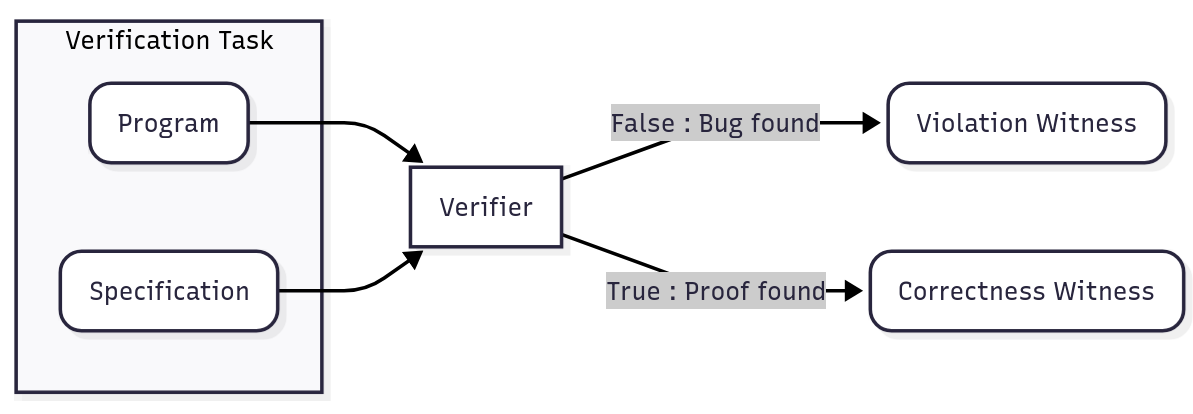
\includegraphics[width=1\textwidth]{figures/verifier.png}
  \caption{Verificatoin}
  \label{fig:Verification}
\end{figure}

% ---
% config:
%       theme: redux
% ---

% flowchart LR
%   subgraph Verification Task
%     Program[Program]
%     Specification[Specification]
%   end

%   Program --> Verifier
%   Specification --> Verifier

%   Verifier -->|False : Bug found| ViolationWitness[Violation Witness]
%   {Verifier -->|True : Proof found| CorrectnessWitness[Correctness Witness]}
  
\section{Witness-based Result Validation}
Witnesses generated by different tools are typically cross-checked to ensure accuracy. 
A witness, being structured data in a standard format, facilitates faster result validation
across various tools compared to a complete reverification. While verification and validation 
are often confused, validation specifically relies on a witness, which offers additional 
information about the program's verification process. Witnesses accelerate this process by 
providing precomputed verification data. Furthermore, they enable the validation of results 
obtained from other tools.

\begin{figure}[h]
  \centering
  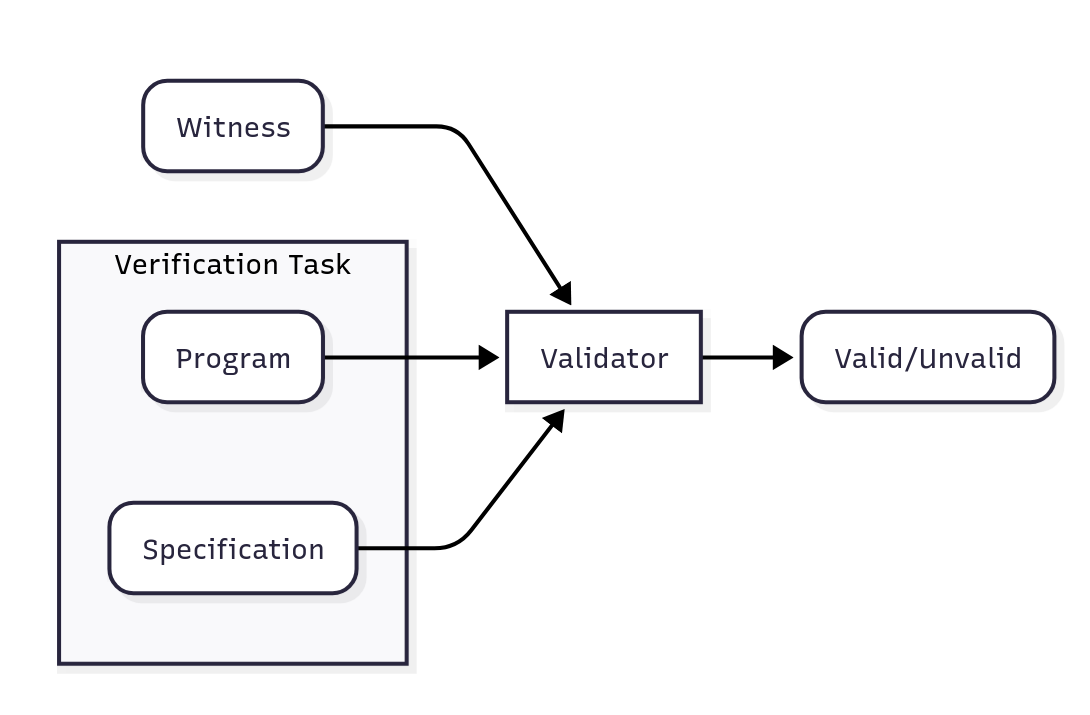
\includegraphics[width=0.8\textwidth]{figures/validator.png}
  \caption{Validation}
  \label{fig:Validation}
\end{figure}

% ---
% config:
%   theme: redux
%   layout: dagre
% ---
% flowchart LR
%  subgraph subGraph0["Verification Task"]
%         P("Program")
%         S("Specification")
%   end
%     W("Witness") --> V["Validator"]
%     P --> V
%     S --> V
%     V --> C("Valid/Unvalid")

\section{CFA}

To perform model checking, a program written in source code must first be transformed into a formal model. 
The formal model used in the Theta validator built is an Control-Flow Automaton (CFA).

\begin{definition}[Control-flow automata] Let:
\begin{itemize}
  \item $v :=$ variable
  \item $D_v :=$ domain of variable $v$
  \item $\varphi$ is an expression $\Rightarrow \mathrm{var}(\varphi) = \{\forall v \mid v \in \varphi\}$
  \item $\text{predicate} := p: D_{v_i} \times \dots \times D_{v_n} \to \{\text{true}, \text{false}\}$
\end{itemize}
A control-flow automaton is a tuple $\mathrm{CFA} = (V, L, l_0, E)$ where:
\begin{itemize}
  \item $V := \{v_1, \dots, v_n \mid \mathrm{domain}(v_i) = D_{v_i} \}$
  \item $L := \{$program locations modeling the program counter$\}$
  \item $l_0 \in L :=$ initial program location
  \item $E \subseteq L \times \mathrm{Ops} \times L := \{$directed edges representing operations$\}$
  \item $\mathrm{Ops} = \{ \mathrm{op} \mid \mathrm{op} = \text{assignment} \lor \mathrm{op} = \text{assumption} \}$
  \begin{itemize}
    \item $\text{assignment} := (v := \varphi)$ s.t. $v \in V \land \varphi \in D_v \land \mathrm{var}(\varphi) \subseteq V$
    \item $\text{assumption} := [\varphi]$ s.t. $\varphi := \text{predicate} \land \mathrm{var}(\varphi) \subseteq V$
  \end{itemize}
\end{itemize}
\end{definition}


Evidently, a Control Flow Automaton (CFA) is a formalism based on graphs. 
Furthermore, assignment and assumption statements can be represented as transition functions, 
making them applicable in model checking.
\begin{align}
\mathrm{tran}\bigl(v := \varphi\bigr)
&\;=\;
\bigl(v' = \varphi\bigr)
\;\land\;
\bigwedge_{\,u \in V \setminus \{v\}} (u' = u),
\\
\mathrm{tran}\bigl([\psi]\bigr)
&\;=\;
\psi
\;\land\;
\bigwedge_{\,v \in V} (v' = v).
\end{align}

Although the validator we developed in Theta uses the concept of a Control Flow Automaton (CFA) as 
defined here, it actually employs an Extended Control Flow Automaton (XCFA). The XCFA is simply 
a more comprehensive version of a CFA designed to manage more intricate processes. However, in 
our current implementation, we don't utilize any of the additional capabilities offered by the XCFA.



\section{Product Automaton and Multianalysis}
Another formalism we'll need to understand is the Product Automaton. The intuition behind its 
importance lies in its ability to represent the combination of different formalism. We 
often model individual systems separately, but we need a way to understand their combined behavior, 
or what happens when these models interact in a defined manner. Informally, a Product 
Automaton is precisely this: the result of combining two formalisms. Multi-analysis, then,
is the analysis performed on this resulting Product Automaton. While you can theoretically 
combine any two formalisms, in our specific case, we're interested in the product automaton 
of two CFAs.

% More precisely:
% \begin{definition}[Product Automaton of CFA's]
% Given two CFAs:
% \begin{itemize}
%     \item $\text{CFA}_1 = (V_1, L_1, l_{0_1}, E_1)$
%     \item $\text{CFA}_2 = (V_2, L_2, l_{0_2}, E_2)$
% \end{itemize}
% with $V_1 \cap V_2 = \emptyset$ (disjoint variables), their \textbf{product automaton} is defined as:
% \[
% \text{CFA}_1 \times \text{CFA}_2 = (V, L, l_0, E)
% \]
% where:
% \begin{itemize}
%     \item $V = V_1 \cup V_2$ (combined variables)
%     \item $L = L_1 \times L_2$ (product locations: pairs $(l_1, l_2)$ where $l_1 \in L_1, l_2 \in L_2$)
%     \item $l_0 = (l_{0_1}, l_{0_2})$ (initial location)
%     \item $E \subseteq L \times \mathrm{Ops} \times L$ (transitions defined below)
% \end{itemize}

% \noindent The edge set $E$ is constructed as follows:
% \begin{itemize}
%     \item \textbf{Synchronized transitions}:
%     \begin{itemize}
%         \item For edges $(l_1, [\varphi_1], l_1') \in E_1$ and $(l_2, [\varphi_2], l_2') \in E_2$:
%         \[
%         \big((l_1, l_2), [\varphi_1 \land \varphi_2], (l_1', l_2')\big) \in E \quad \text{if } \varphi_1 \land \varphi_2 \text{ is satisfiable}
%         \]
%         \item For $(l_1, (v := \varphi), l_1') \in E_1$ and $(l_2, [\psi], l_2') \in E_2$:
%         \[
%         \big((l_1, l_2), (v := \varphi), (l_1', l_2)\big) \in E \quad \text{if } \psi \text{ holds after the assignment}
%         \]
%         (Analogously for assignments in $\text{CFA}_2$ and assumptions in $\text{CFA}_1$)
%     \end{itemize}
    
%     \item \textbf{Interleaved transitions}:
%     \begin{itemize}
%         \item For any edge $(l_1, \mathrm{op}, l_1') \in E_1$:
%         \[
%         \big((l_1, l_2), \mathrm{op}, (l_1', l_2)\big) \in E \quad \forall l_2 \in L_2
%         \]
%         \item For any edge $(l_2, \mathrm{op}, l_2') \in E_2$:
%         \[
%         \big((l_1, l_2), \mathrm{op}, (l_1, l_2')\big) \in E \quad \forall l_1 \in L_1
%         \]
%     \end{itemize}
% \end{itemize}
% \end{definition}


\section{Witness Validation on other Tools}


% https://ftsrg.mit.bme.hu/phd-thesis-hajdua/dissertation.pdf
% page 1
% page 46 control flow automata
% https://link.springer.com/chapter/10.1007/978-3-031-66149-5_11
% Stair, Ralph M. (2003). Principles of Information Systems, Sixth Edition. Thomson. p. 16. ISBN 0-619-06489-7. "Software consists of computer programs that govern the operation of the computer."

